\documentclass[12pt, a4paper, UTF8, fontset=windows]{ctexbook}
\usepackage{amsmath, amsthm, amssymb, amsfonts, bm, color, fancyhdr, framed, geometry, graphicx, hyperref, lastpage, listings, mathrsfs, xcolor}


\linespread{1.5}
\definecolor{shadecolor}{RGB}{241, 241, 255}
\newcounter{problemname}
\newenvironment{problem}{\begin{shaded}\stepcounter{problemname}\par\noindent\textbf{Q\arabic{problemname}.}}{\end{shaded}\par}
\newenvironment{solution}{\par\noindent\textbf{Ans.}}{\par}

\geometry{left=20mm,right=20mm, top=20mm, bottom=22mm} % 页边距
\setlength{\headheight}{15pt}
\pagestyle{fancy} % 设置页脚页眉
\rhead{Assignment4} % 页眉右边
% \noindent % 取消首段缩进

\definecolor{mygreen}{rgb}{0,0.6,0}
\definecolor{mygray}{rgb}{0.5,0.5,0.5}
\definecolor{mymauve}{rgb}{0.58,0,0.82}
% 代码设置
\lstset{ 
backgroundcolor=\color{white},      % choose the background color
basicstyle=\footnotesize\ttfamily,  % size of fonts used for the code
columns=fullflexible,
tabsize=4,
breaklines=true,               % automatic line breaking only at whitespace
captionpos=b,                  % sets the caption-position to bottom
commentstyle=\color{mygreen},  % comment style
keywordstyle=\color{blue},     % keyword style
stringstyle=\color{mymauve}\ttfamily,  % string literal style
frame=single,
rulesepcolor=\color{red!20!green!20!blue!20},
language=c++,
xleftmargin=3em,
xrightmargin=3em
}


\begin{document}

\cfoot{\thepage\ / \pageref{LastPage}} % 页眉中间位添加内容:页码/总页码

\thispagestyle{empty}

\begin{figure}[t]
    \centering
    
\includegraphics[width=6cm]{../../src/images/logo.jpg}
\end{figure}

\vspace*{\fill}
    \begin{center}
        \Huge\textbf{Assignment4}
    \end{center}
\vspace*{\fill}

\begin{table}[b]
    \centering
    \large
    \begin{tabular}{ll}
    \textbf{课程:} & 数据库原理与应用 \\
    \textbf{姓名:} & 雷翔 \\
    \textbf{学号:} & 2053932 \\
    \textbf{时间:} & 2023年6月 \\
    \end{tabular}
\end{table}


\newpage

\setcounter{page}{1} % 页码从当前页开始

\begin{problem}
    13.14 标准的缓沖区管理器假定每个块的大小和读取代价都是相同的。设想一个缓冲区管理器使用对象引用率而不是 LRU,
    对象引用率是指一个对象在此前的n秒内被访问的频率。假设我们要在缓冲区中存储变长和读取代价可变(例如网页,它的读取代价取决于它从哪个站点被获取)
    的对象。试建议缓冲区管理器可以如何选择要从缓冲区中移出哪个块。
\end{problem}

\begin{solution}

    维护一个优先队列,优先级取决于以下三个因素:
    
    对象引用率X、对象大小Y、对象读取代价Z。

    记 T = $k_1 \times X$ + $k_2 \times Y$ + $k_3 \times Z$,其中 $k_1, k_2, k_3$ 为常数。 

    每次缓冲区满时,将优先级最低的对象,即 T 最小的对象移出缓冲区。
    
\end{solution}

\newpage

\begin{problem}
    14.3 用下面的码值集合建立一棵 $B^+$ 树:

    (2, 3, 5, 7, 11, 17, 19, 23, 29, 31)

    假设树初始为空,按升序添加这些值。当一个节点所能容纳的指针数是下列情况时,请分别构造 $B^+$ 树:

    a. 4 b. 6 c. 8
\end{problem}

\begin{solution}

a.

n = 4,每个叶节点最多有 $n - 1 = 3$ 个值,最少有 $\lceil (n-1)/2 \rceil - 1 = 2$ 个值。

    \begin{figure}[htb]
        \centering
        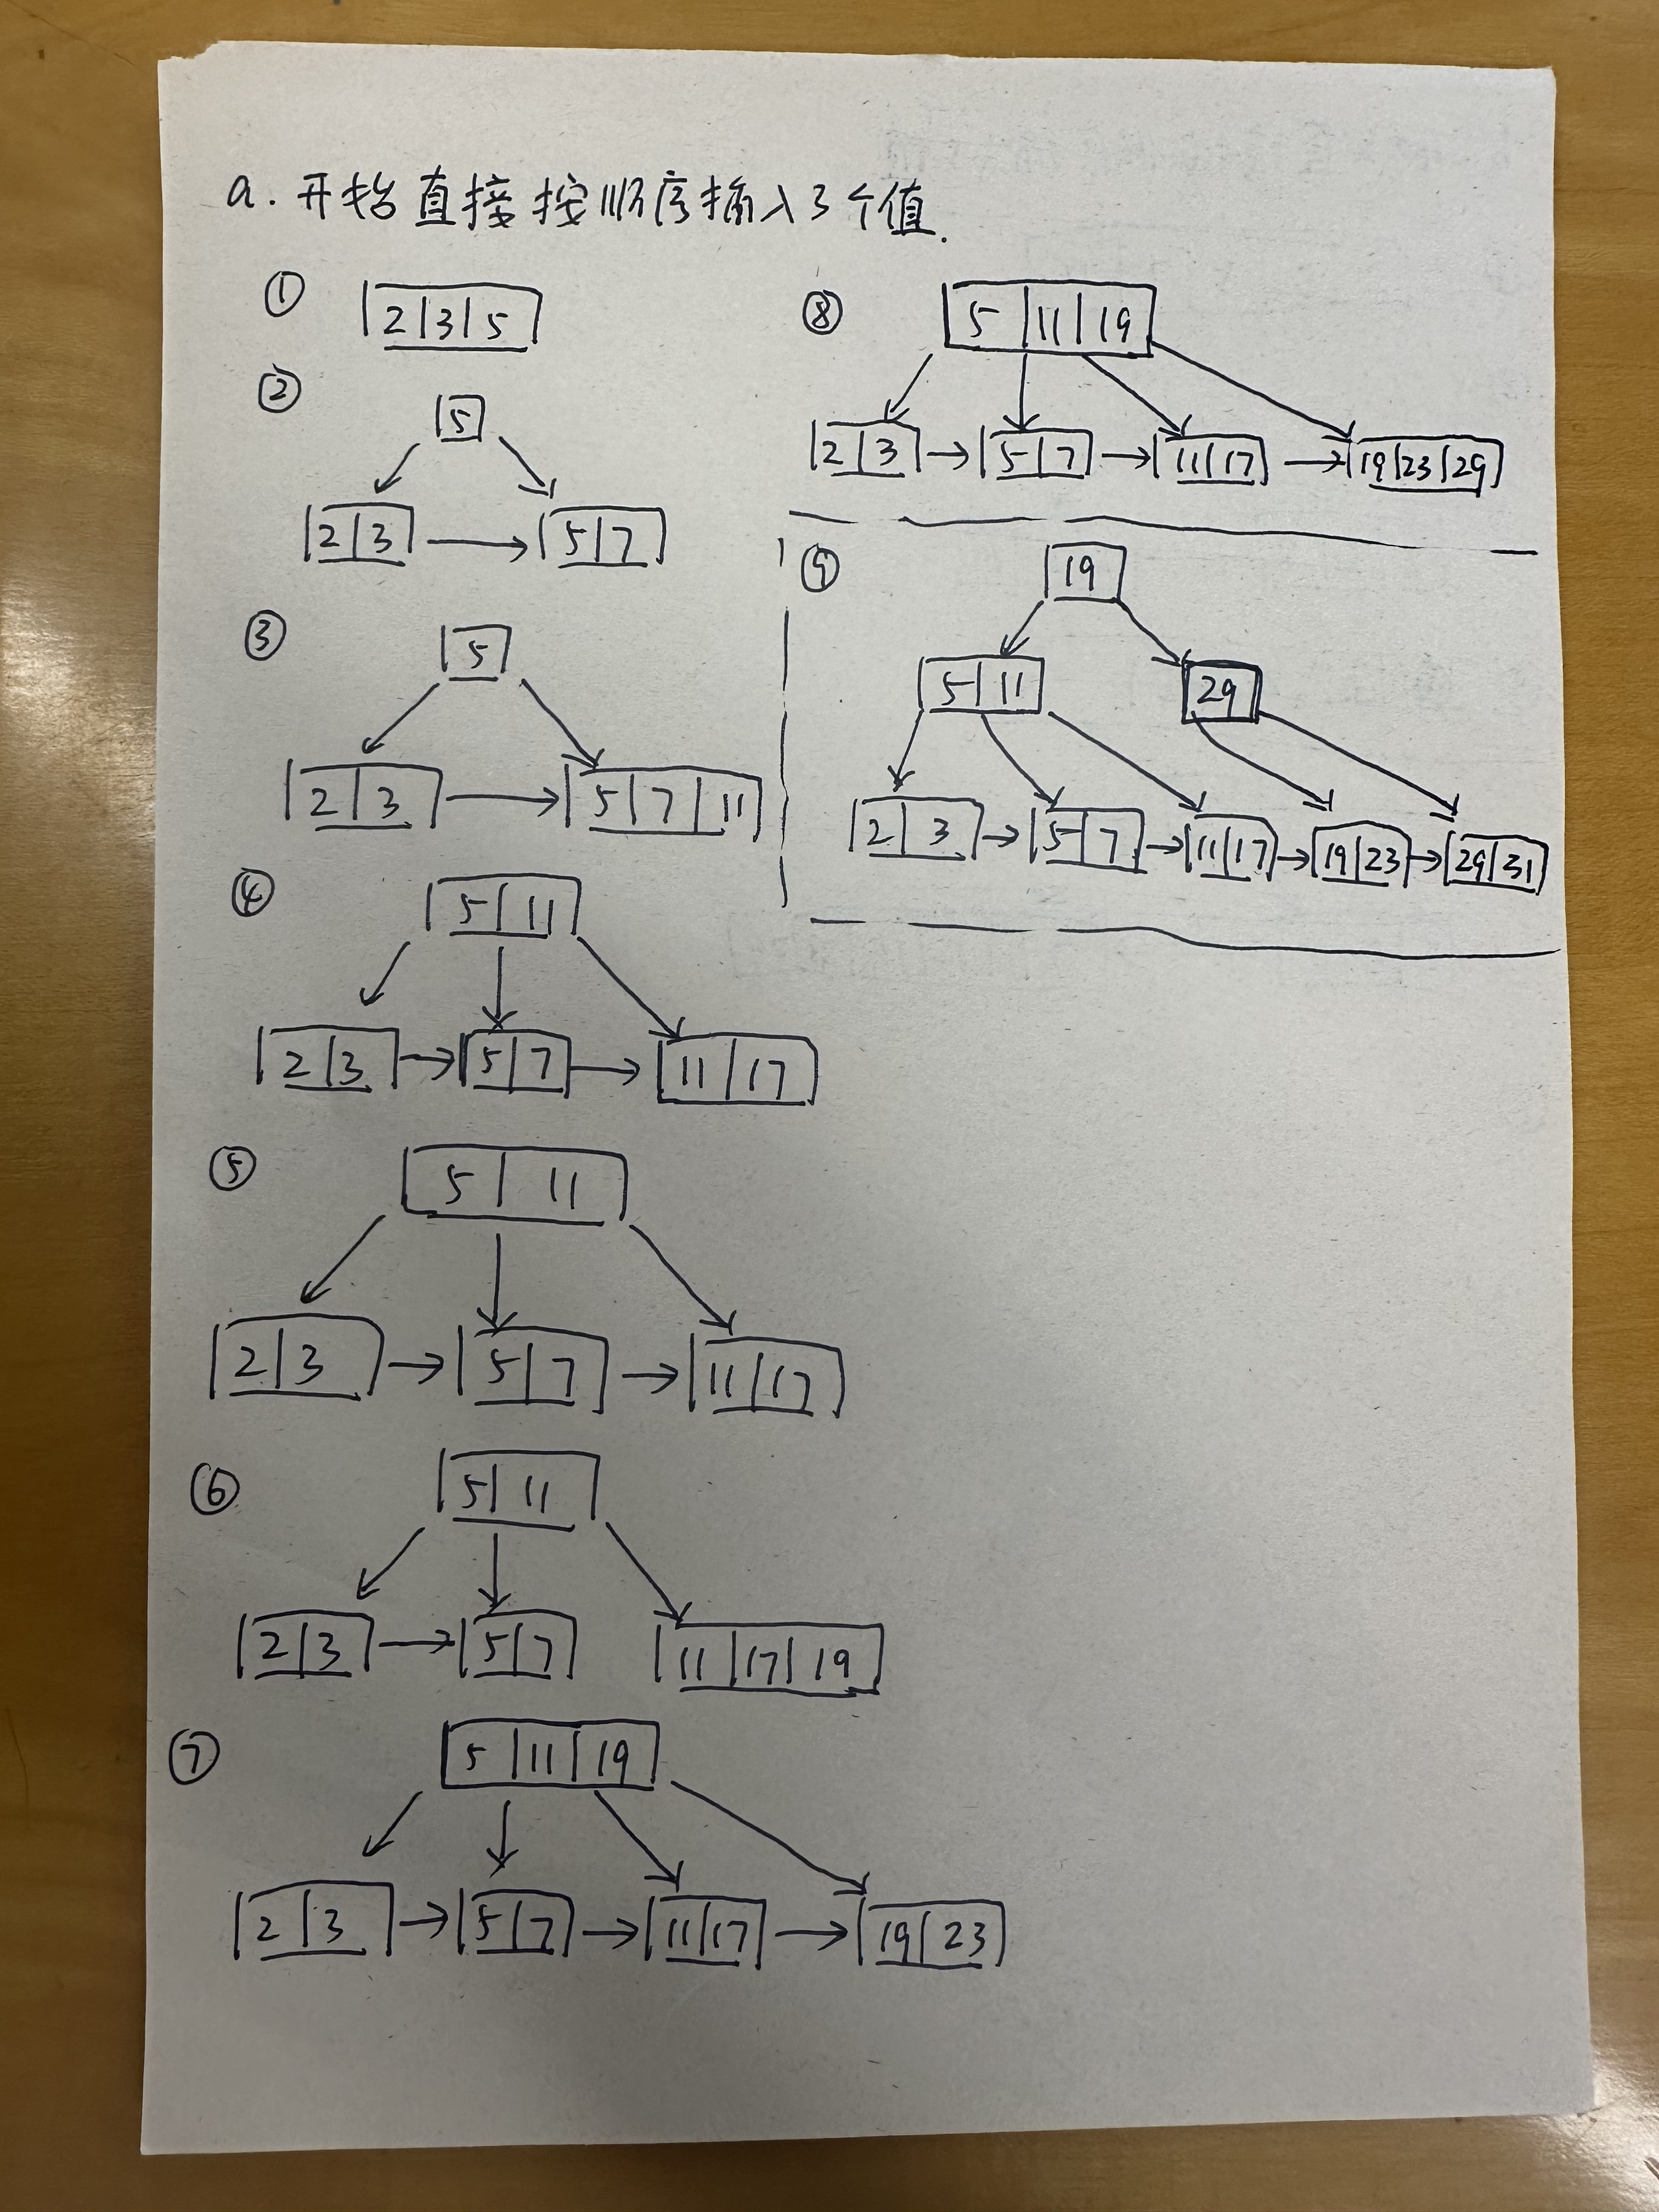
\includegraphics[width=9cm]{../../src/images/hw4-Q2-a.jpg}
    \end{figure}

\newpage

b.

n = 6,每个叶节点最多有 $n - 1 = 5$ 个值,最少有 $\lceil (n-1)/2 \rceil - 1 = 3$ 个值。

    \begin{figure}[htb]
        \centering
        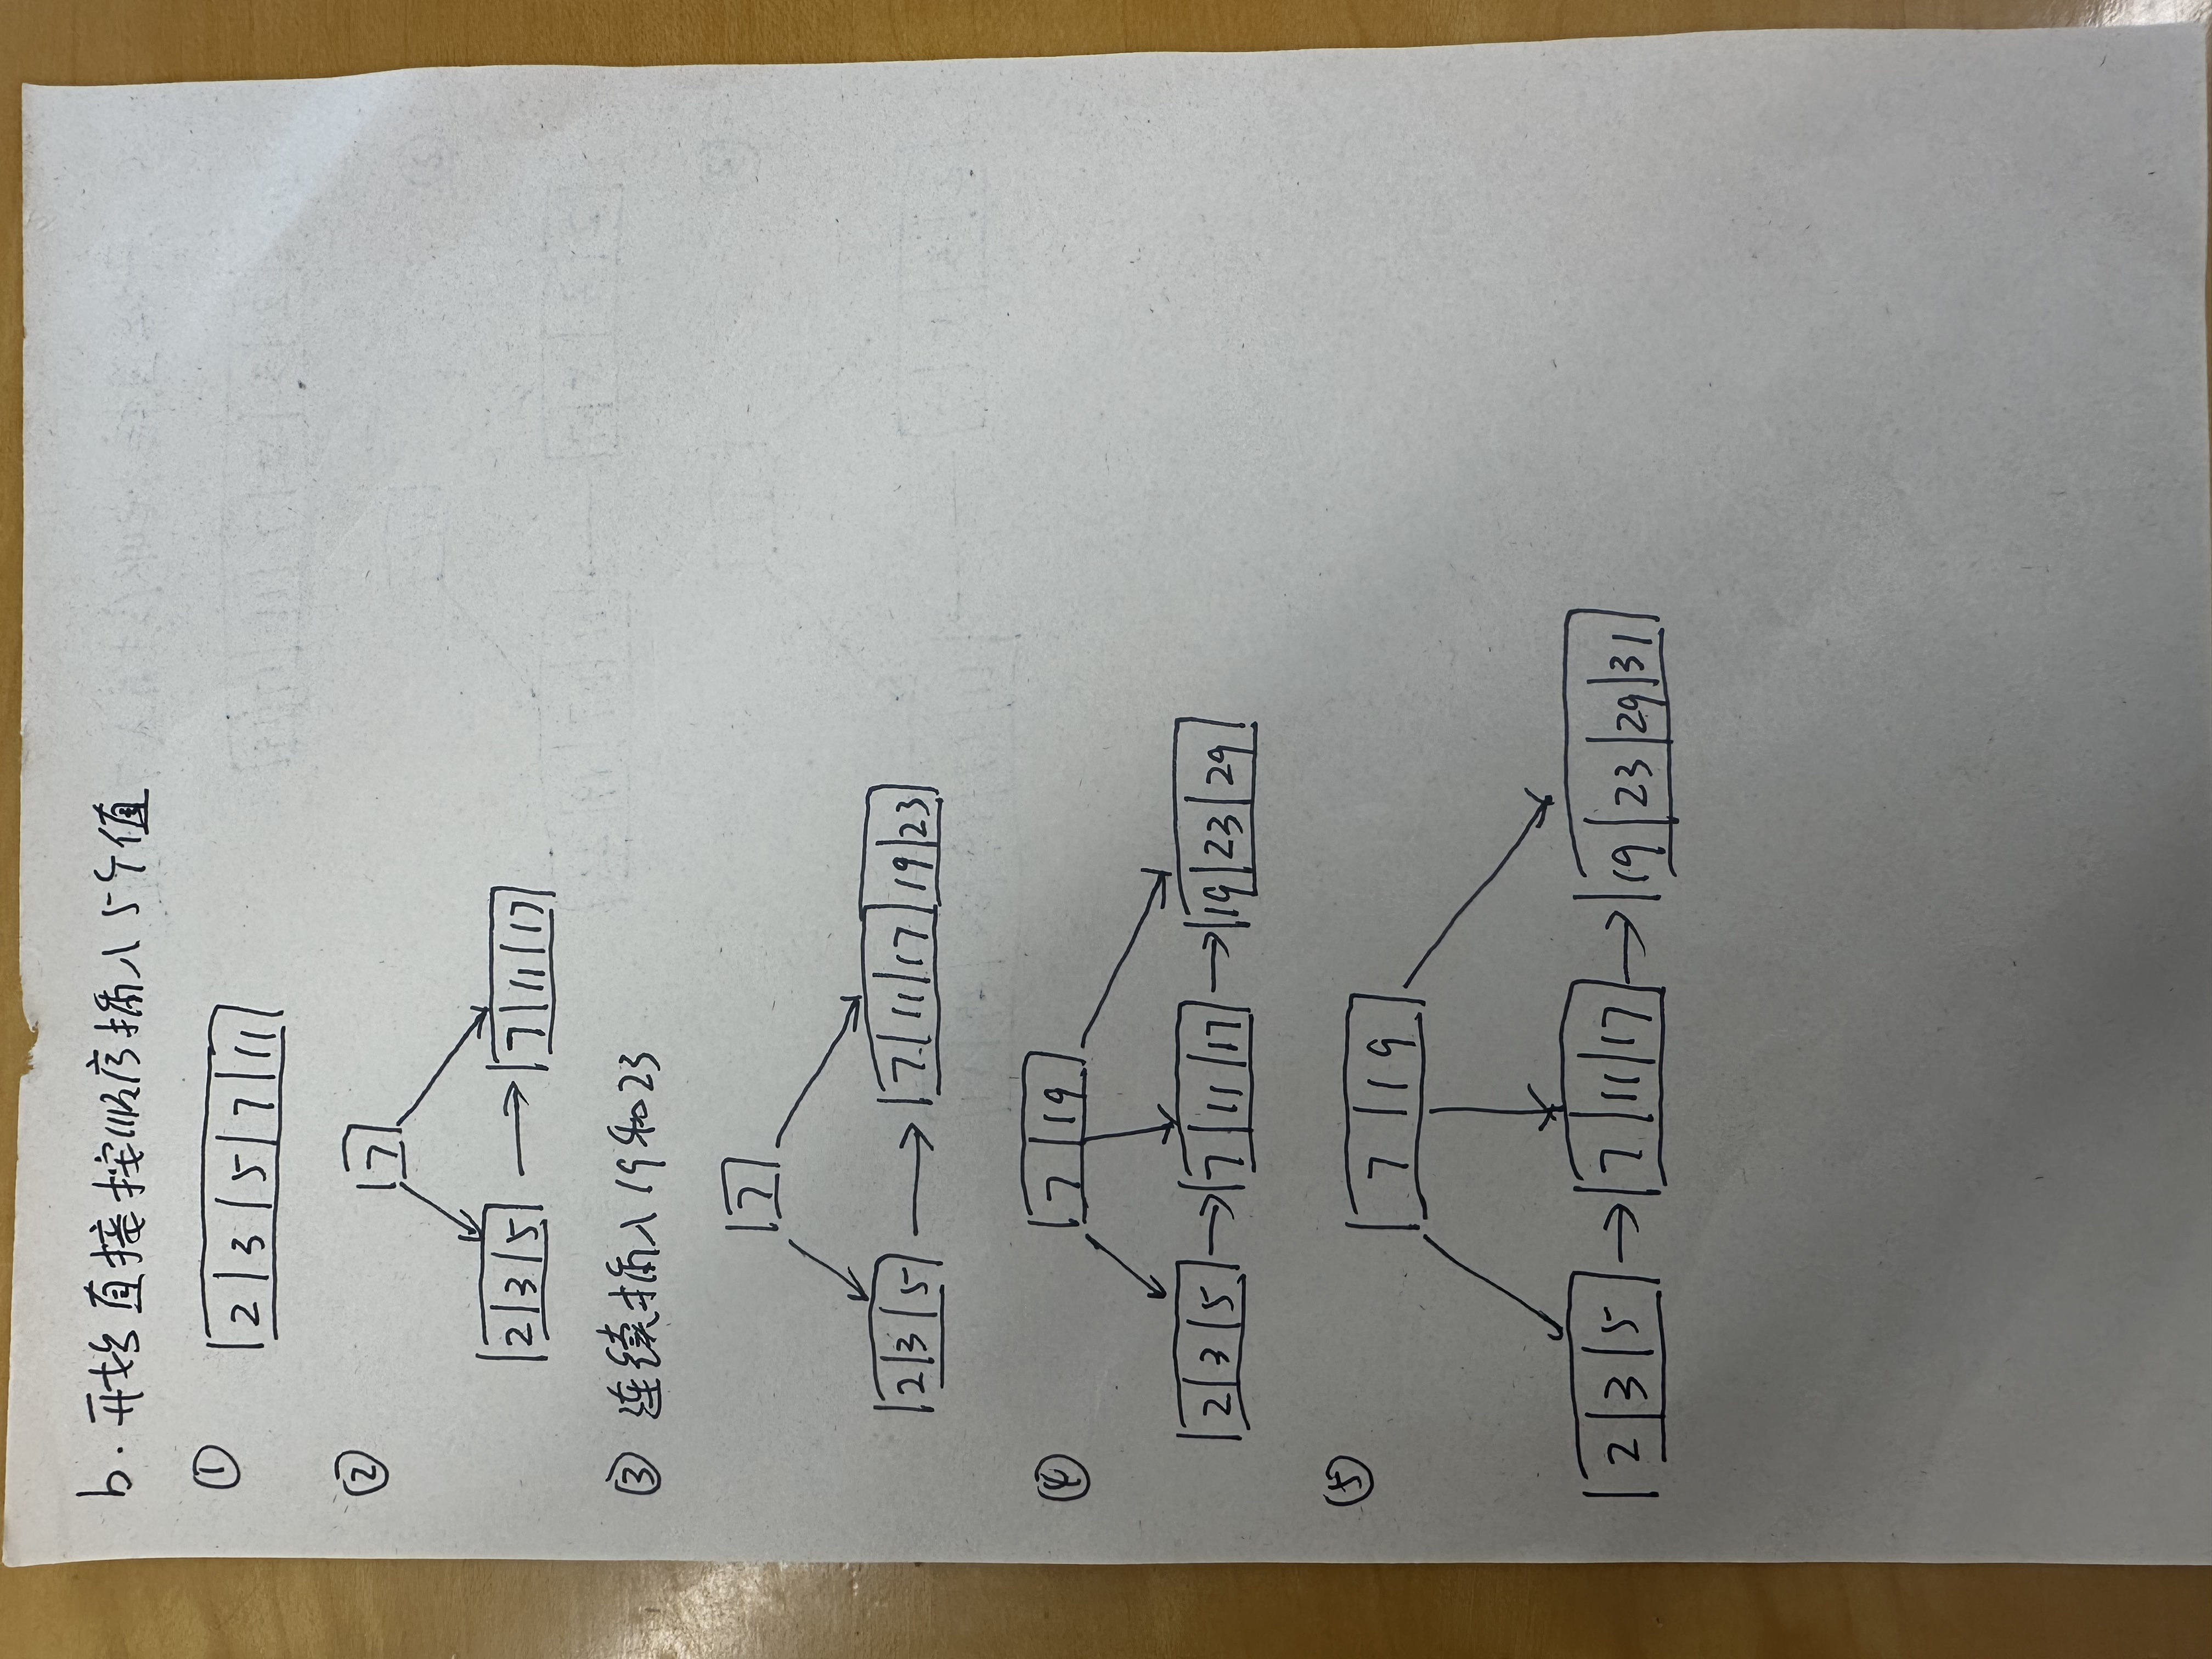
\includegraphics[width=9cm, angle=-90]{../../src/images/hw4-Q2-b.jpg}
    \end{figure}


c.

n = 8,每个叶节点最多有 $n - 1 = 7$ 个值,最少有 $\lceil (n-1)/2 \rceil - 1 = 4$ 个值。

    \begin{figure}[htb]
        \centering
        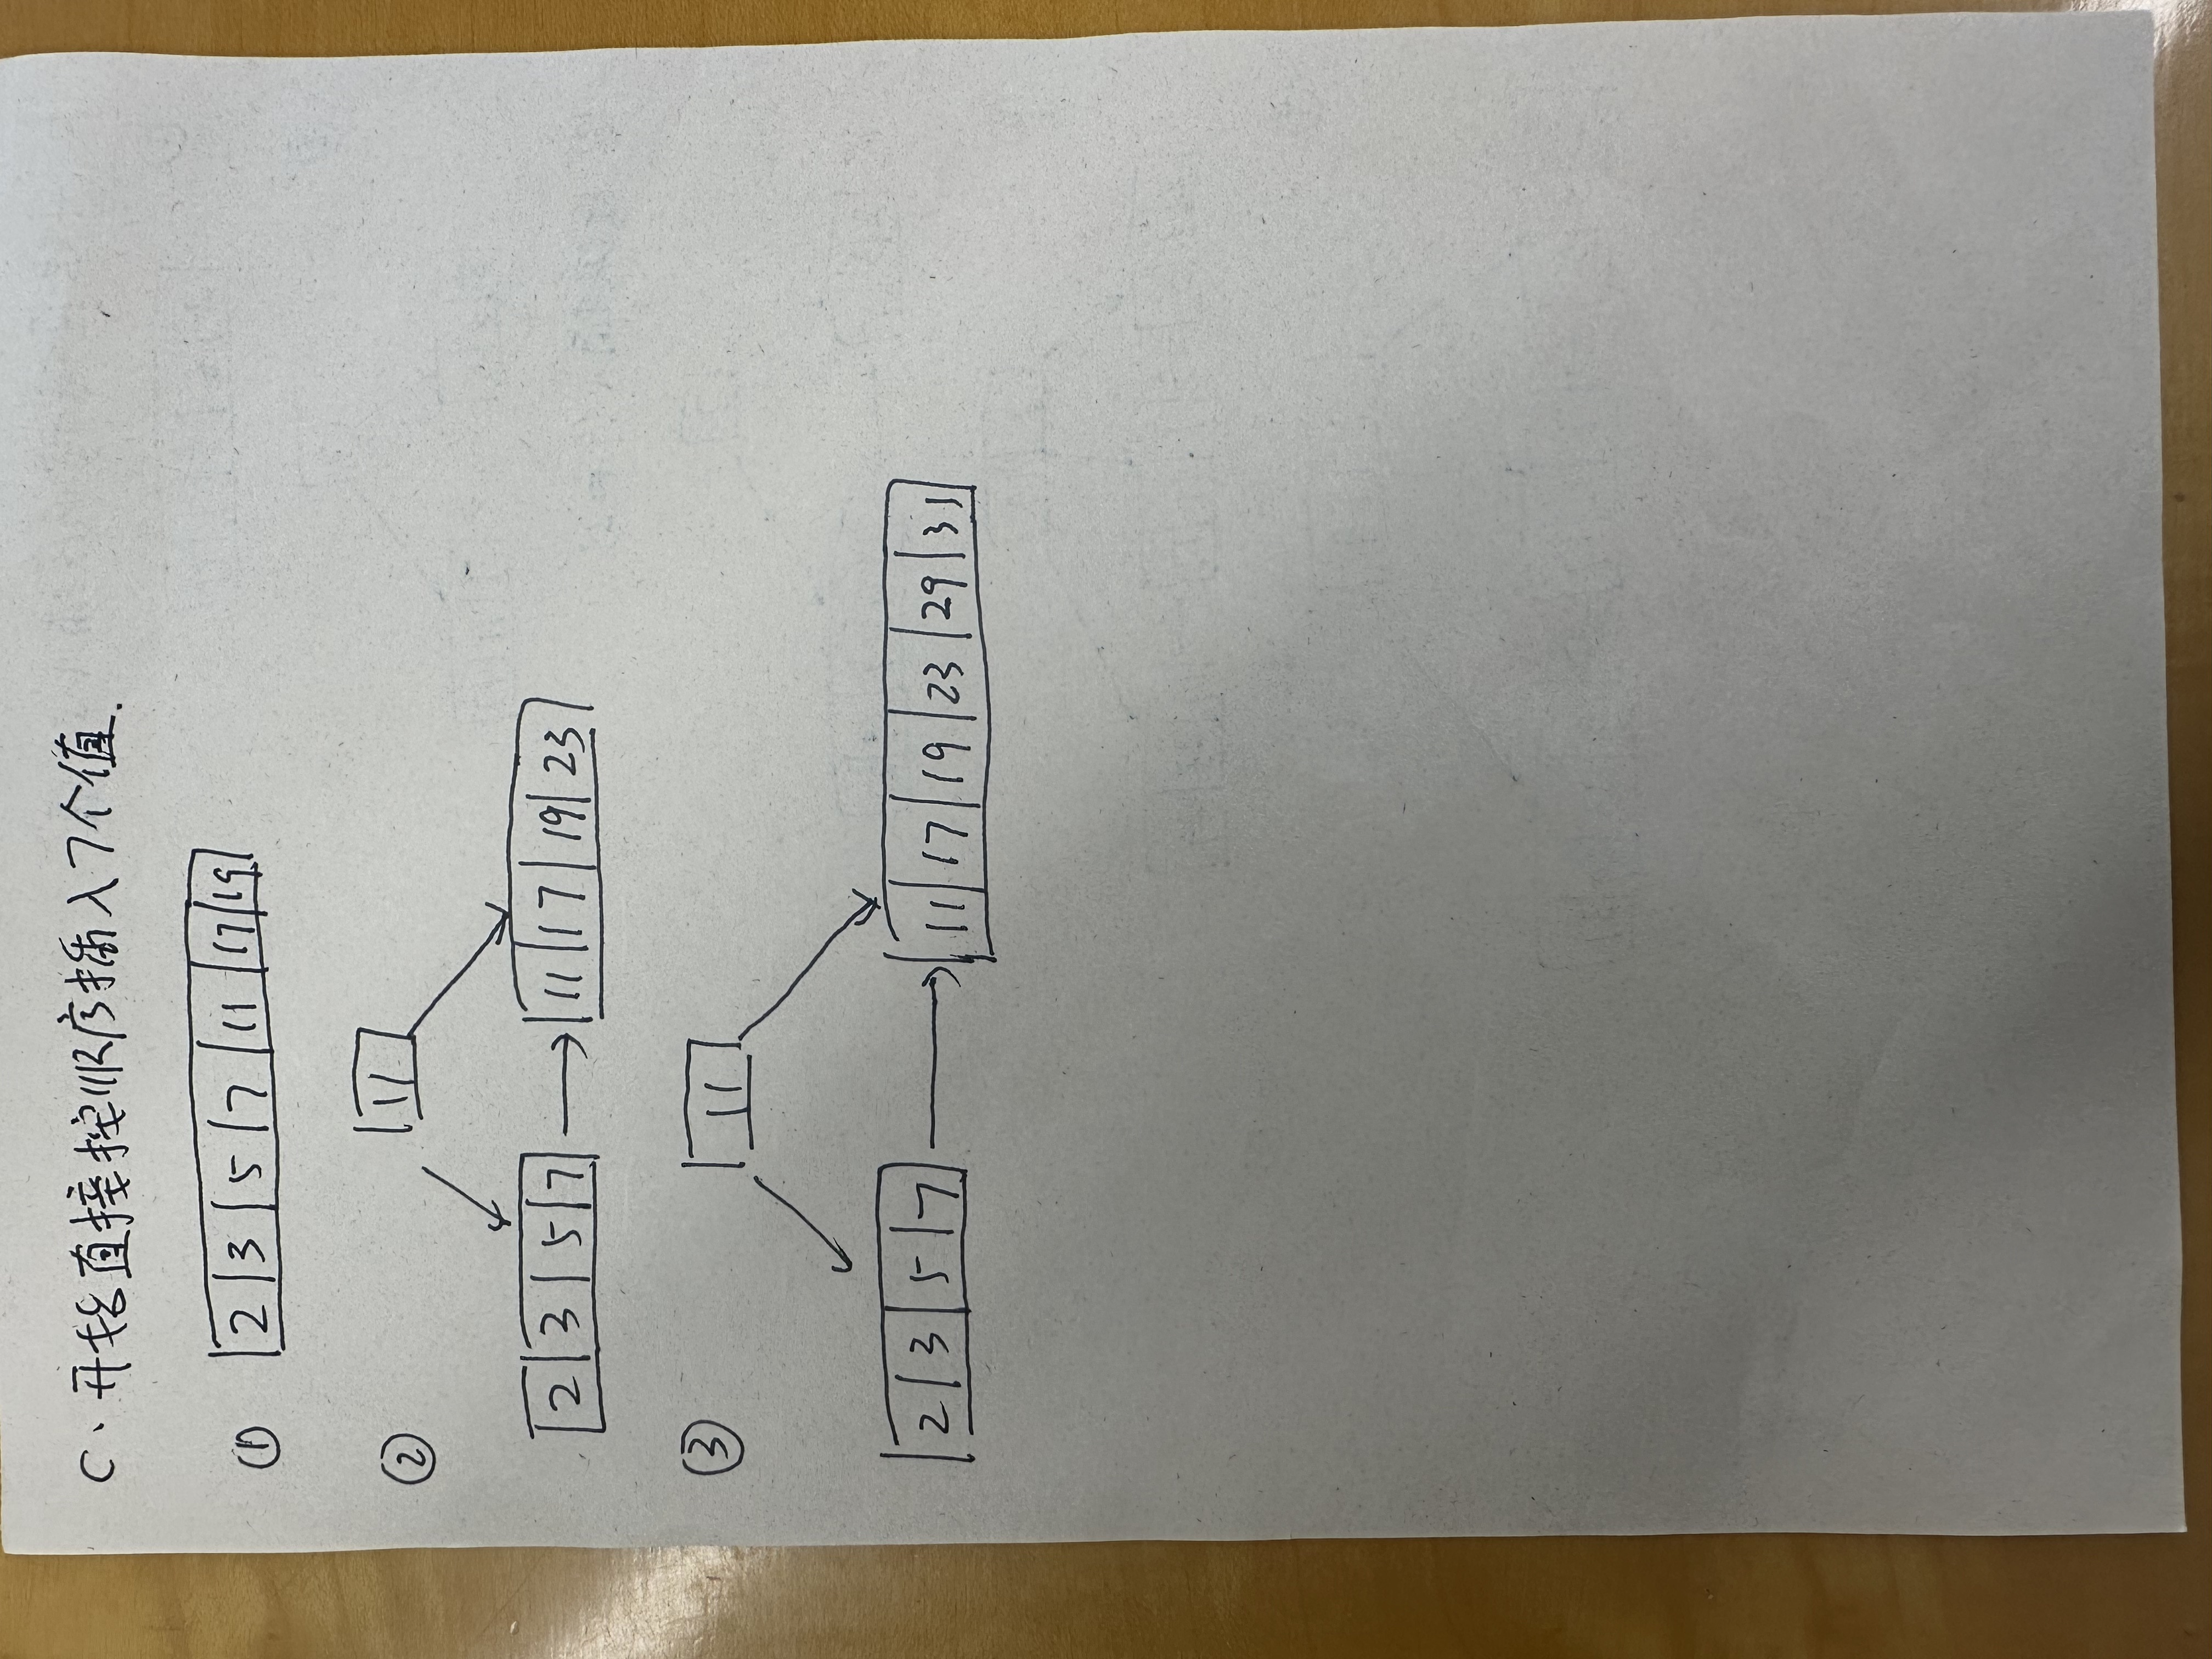
\includegraphics[width=9cm, angle=-90]{../../src/images/hw4-Q2-c.jpg}
    \end{figure}

\end{solution}

\newpage

\begin{problem}
    14.13 请考虑如图14-1所示的 instructor 关系。
    
    a. 在 salary 属性上构建一个位图索引,把 salary 的值分为 4 个区间:小于 50000 的,50000 到 60000 以下的,
    60000 到 70000 以下的,70000 及以上的。

    b. 请考虑一个查询:查找在金融系中工资为 80000 或更高的所有教师。概述回答该查询的步骤,并给出为回答这个查询而
    构建的最终位图和中间位图。    
\end{problem}
    

\begin{solution}
    \begin{figure}[htb]
        \centering
        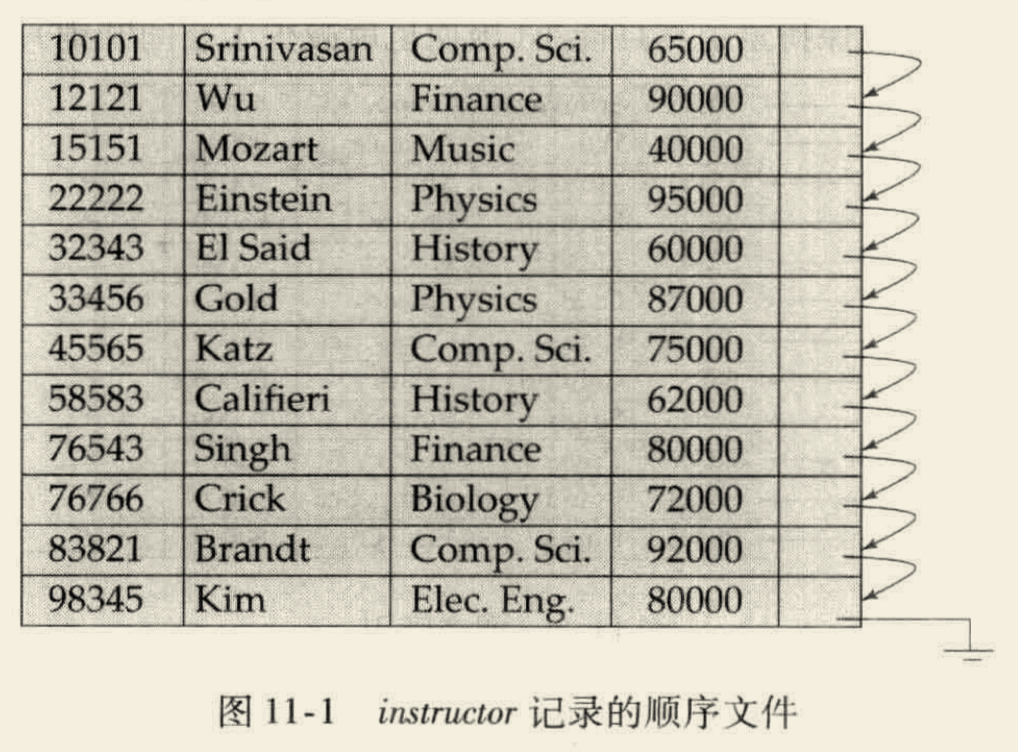
\includegraphics[width=0.8\textwidth]{../../src/images/hw4-Q3.png}
    \end{figure}

a. 

记 $L_1$ 为小于 50000 的,$L_2$ 为 50000 到 60000 以下的,$L_3$ 为 60000 到 70000 以下的,$L_4$ 为 70000 及以上的。

\begin{table}[h]
    \centering
    \begin{tabular}{|c|c|}
        \hline
        $L_1$ & 0 0 1 0 0 0 0 0 0 0 0 0
        \\ \hline
        $L_2$ & 0 0 0 0 0 0 0 0 0 0 0 0
        \\ \hline
        $L_3$ & 1 0 0 0 1 0 0 1 0 0 0 0
        \\ \hline
        $L_4$ & 0 1 0 1 0 1 1 0 1 1 1 1
        \\ \hline
    \end{tabular}

    \caption{salary 的位图索引}
\end{table}

\newpage 

b.

记 $A_1$ 为金融系,$A_2$ 为非金融系。

\begin{table}[h]
    \centering
    \begin{tabular}{|c|c|}
        \hline
        $A_1$ & 0 1 0 0 0 0 0 0 1 0 0 0
        \\ \hline
        $A_2$ & 1 0 1 1 1 1 1 1 0 1 1 1
        \\ \hline
    \end{tabular}

    \caption{dept\_name 的位图索引}
\end{table}

记 $B_1$ 为工资低于 80000 的,$B_2$ 为工资高于 80000 的。

\begin{table}[h]
    \centering
    \begin{tabular}{|c|c|}
        \hline
        $B_1$ & 1 0 1 0 1 0 1 1 0 1 0 0 
        \\ \hline
        $B_2$ & 0 1 0 1 0 1 0 0 1 0 1 1
        \\ \hline
    \end{tabular}

    \caption{salary 的位图索引}
\end{table}

取 dept\_name 为 $A_1$ 的位图和 salary 为 $B_2$ 位图,并执行这两个位图的交,得到最终位图。

\begin{table}[h]
    \centering
    \begin{tabular}{|c|c|}
        \hline
        $A_1 \cap B_2$ & 0 1 0 0 0 0 0 0 1 0 0 0 
        \\ \hline
    \end{tabular}

    \caption{最终位图}
\end{table}

所以,金融系中工资为 80000 或更高的所有教师有 2 个,分别是 Wu 和 Singh。
 
\end{solution}

\newpage 

\begin{problem}
    17.15 请考虑以下两个事务:

    $T_{13}$ : 
    \begin{lstlisting}
        read(A);
        read(B);
        if A = 0 then B := B + 1;
        write(B);
    \end{lstlisting}

    $T_{14}$ : 
    \begin{lstlisting}
        read(B);
        read(A);
        if B = 0 then A := A + 1;
        write(A);
    \end{lstlisting}

    令一致性需求为 $A=0 ~V~ B=0$,初值是 A=B=0。
    
    a. 请说明包括这两个事务的每一个串行执行都保持了数据库的一致性。

    b. 请给出 $T_{13}$ 和 $T_{14}$ 的一个并行执行,它产生了不可串行化的调度。

    c. 存在产生可串行化调度的 $T_{13}$ 和 $T_{14}$ 的并行执行吗?
\end{problem}


\begin{solution}
a. 

一致性需求是 A、B 至少有一个为 0,初始条件为 A=B=0

假设两个事务以先 $T_{13}$ 后 $T_{14}$ 的次序执行,执行顺序如下表所示:

\begin{table}[h]
    \centering
    \begin{tabular}{|c|c|} \hline
        $T_{13}$ & $T_{14}$  \\ \hline
        read(A) &  \\ \hline
        read(B) &  \\ \hline
        if A = 0 then B := B + 1 &  \\ \hline
        write(B) &  \\ \hline
        & read(B) \\ \hline
        & read(A) \\ \hline
        & if B = 0 then A := A + 1 \\ \hline
        & write(A) \\ \hline
    \end{tabular}
\end{table}

执行完成后,A=0、B=1,保持数据库的一致性。

\newpage

同理,假设两个事务以先 $T_{14}$ 后 $T_{13}$ 的次序执行,执行顺序如下表所示:

\begin{table}[h]
    \centering
    \begin{tabular}{|c|c|} \hline
        $T_{13}$ & $T_{14}$  \\ \hline
        & read(B) \\ \hline
        & read(A) \\ \hline
        & if B = 0 then A := A + 1 \\ \hline
        & write(A) \\ \hline
        read(A) &  \\ \hline
        read(B) &  \\ \hline
        if A = 0 then B := B + 1 &  \\ \hline
        write(B) &  \\ \hline
    \end{tabular}
\end{table}

执行完成后,A=1、B=0,保持数据库的一致性。

b. 

\begin{table}[h]
    \centering
    \begin{tabular}{|c|c|} \hline
        $T_{13}$ & $T_{14}$  \\ \hline
        read(A) &  \\ \hline
        read(B) &  \\ \hline
        & read(B)  \\ \hline
        & read(A) \\ \hline
        if A = 0 then B := B + 1 &  \\ \hline
        & if B = 0 then A := A + 1 \\ \hline
        write(B) &  \\ \hline
        & write(A) \\ \hline
    \end{tabular}
\end{table}

执行完成后,A=1、B=1,没有保持数据库的一致性,产生了不可串行化的调度。

c.

一旦 $T_{13} $和 $T_{14}$ 并行执行,那么必然导致先进行所有的读取操作,才会进行写操作,因为要并行,所以大体存在两种情况:

情况一:先进行 $T_{13}$,在 $T_{13}$ 进行写操作前,$T_{14}$ 进行读。

情况二:先进行 $T_{14}$,在 $T_{14}$ 进行写操作前,$T_{13}$ 进行读。

无论哪种情况,因为写操作还没有完成,读到的都是0,所以两个if then语句均会执行,最后的结果就是A=1、B=1,不满足一致性

所以不存在产生可串行化调度的 $T_{13}$ 和 $T_{14}$ 的并行执行。

\end{solution}

\end{document}